%\title{LaTeX Portrait Poster Template}
%%%%%%%%%%%%%%%%%%%%%%%%%%%%%%%%%%%%%%%%%
% a0poster Portrait Poster
% LaTeX Template
% Version 1.0 (22/06/13)
%
% The a0poster class was created by:
% Gerlinde Kettl and Matthias Weiser (tex@kettl.de)
%
% This template has been downloaded from:
% http://www.LaTeXTemplates.com
%
% License:
% CC BY-NC-SA 3.0 (http://creativecommons.org/licenses/by-nc-sa/3.0/)
%
%%%%%%%%%%%%%%%%%%%%%%%%%%%%%%%%%%%%%%%%%

%----------------------------------------------------------------------------------------
%	PACKAGES AND OTHER DOCUMENT CONFIGURATIONS
%----------------------------------------------------------------------------------------

\documentclass[a0,portrait]{a0poster}

\usepackage{multicol} % This is so we can have multiple columns of text side-by-side
\columnsep=100pt % This is the amount of white space between the columns in the poster
\columnseprule=3pt % This is the thickness of the black line between the columns in the poster

\usepackage[svgnames]{xcolor} % Specify colors by their 'svgnames', for a full list of all colors available see here: http://www.latextemplates.com/svgnames-colors

\usepackage{times} % Use the times font
%\usepackage{palatino} % Uncomment to use the Palatino font

\usepackage{graphicx} % Required for including images
\graphicspath{{figures/}} % Location of the graphics files
\usepackage{booktabs} % Top and bottom rules for table
\usepackage[font=small,labelfont=bf]{caption} % Required for specifying captions to tables and figures
\usepackage{amsfonts, amsmath, amsthm, amssymb} % For math fonts, symbols and environments
\usepackage{wrapfig} % Allows wrapping text around tables and figures
\usepackage{sectsty}
\usepackage{algpseudocode}
\newcommand\tab[1][1cm]{\hspace*{#1}}

% For monospaced-font.
% http://nepsweb.co.uk/docs/progfonts.pdf
\usepackage{inconsolata}
\usepackage[T1]{fontenc}
\newcommand{\textincon}[1]{%
{\fontfamily{zi4}\selectfont #1}}

\sectionfont{\fontsize{54}{54}\selectfont}

\begin{document}

%----------------------------------------------------------------------------------------
%	POSTER HEADER
%----------------------------------------------------------------------------------------

% The header is divided into two boxes:
% The first is 75% wide and houses the title, subtitle, names, university/organization and contact information
% The second is 25% wide and houses a logo for your university/organization or a photo of you
% The widths of these boxes can be easily edited to accommodate your content as you see fit

\begin{minipage}[b]{0.75\linewidth}
\veryHuge \color{NavyBlue} \textbf{Using RNN to fix syntax errors in JavaScript files} \color{Black}\\ % Title
\Huge \textit{}\\[2cm] % Subtitle
\huge \textbf{Jordan Siaw, Justin Lew, and Luiz Peres}\\[0.5cm] % Author(s)
\huge SFU School of Computing Science\\[0.4cm] % University/organization
\Large \texttt{[\color{NavyBlue}'jsiaw'\color{Black}, \color{NavyBlue}'jylew'\color{Black}, \color{NavyBlue}'lperesde']\color{Black}.\color[rgb]{0.435, 0.258, 0.756}map\color{Black}(f \color[rgb]{0.843, 0.227, 0.286}=> \color{Black}f \color[rgb]{0.843, 0.227, 0.286}+ \color{NavyBlue}'@sfu.ca'\color{Black})}\\
\end{minipage}
%
\begin{minipage}[b]{0.25\linewidth}

\includegraphics[width=20cm]{logo.png}\\
\end{minipage}

\vspace{1cm} % A bit of extra whitespace between the header and poster content

%----------------------------------------------------------------------------------------

\begin{multicols}{2} % This is how many columns your poster will be broken into, a portrait poster is generally split into 2 columns

%----------------------------------------------------------------------------------------
%	Problem
%----------------------------------------------------------------------------------------

\color{Navy} % Navy color for the abstract
\section*{The Problem}
\LARGE

Parsers often fail miserably in helping to find syntax errors. For example:

\color{Black}
\begin{algorithmic}
\State $1$ \textincon{\textbf{if} (process.argv.length $>$ 3)} \tab \textit{\color{red} // Missing '\{' }\color{Black}
\State $2$ \tab\tab \textincon{console.error(\color{NavyBlue} 'Not enough args!'}\color{Black});
\State $3$ \tab\tab \textincon{process.exit(1);}
\State $4$ \textincon{\}}
\end{algorithmic}

\color{NavyBlue} Error message from Mozilla SpiderMonkey (2016):\\\color{Black}
\begin{tabular}{|p{37cm}}
\tab \textincon{wrong.js:4: SyntaxError: syntax error:}\\
\tab \textincon{wrong.js:4: \}}\\
\tab \textincon{wrong.js:4: \^{}}
\end{tabular}
\\

\color{NavyBlue} Error message from Node.js with Google's V8 engine (2016):\\\color{Black}
\begin{tabular}{|p{37cm}}
\tab \textincon{/path/to/wrong.js:6} \tab \textit{\color{red} // Line 6 doesn't even exist!\color{Black}}\\
\tab \textincon{\});}\\
\tab \textincon{\^{}}\\
\tab \textincon{SyntaxError: Unexpected token \}}
\end{tabular}

%----------------------------------------------------------------------------------------
%	GrammarGuru
%----------------------------------------------------------------------------------------

\color{Navy}
\section*{GrammarGuru}

GrammarGuru is a tool created by Santos et al. (Santos EA et al., 2017) that attempts to address this problem by finding and fixing single token syntax errors, using LSTM language models on 10,000 GitHub repos. GrammarGuru works great for locating token insertions and deletions. However, it doesn't perform so well when a token is substituted, e.g. when a keyword is mistyped: \texttt{functions} instead of \texttt{function}.

%----------------------------------------------------------------------------------------
%	Improving GrammarGuru suggestions
%----------------------------------------------------------------------------------------

\section*{Improving GrammarGuru suggestions}

 We improve GrammarGuru by training a neural network that re-evaluates and re-ranks GrammarGuru's scores by using a modification of the features of the ROSE ranking system (Song and Cohn, 2011):

\color{Black}
\begin{center}
\begin{tabular}{ |c|c|c| }
 \hline
 \textbf{ID} & \textbf{Description}\\
 \hline
 1-4 & n-gram precision, n=1...4\\
 5-8 & n-gram recall, n=1...4 \\
 9-12 & n-gram f-measure, n=1...4 \\
 13 & average n-gram precision per code line\\
 14 & n-gram score at the document level \\
 15-18 & n-gram precision excluding common tokens, n=1...4\\
 19-22 & n-gram recall excluding common tokens, n=1...4\\
 23-26 & n-gram f-measure excluding stopwords, n=1...4\\
 27 & average n-gram precision excluding stopwords, n=1...4\\
 28 & pos distance of $hyp_1$, $hyp_2$ against parser error $\{-1, 0, 1 \}$\\
 29 & which of $hyp_1$, $hyp_2$ equals parser error token $\{ -1, 0, 1\}$\\
 30 & $hyp_1$ and/or $hyp_2$ fix the syntax error $\{ -1, 0, 1\}$ \\
 31 & which of $hyp_1$, $hyp_2$ has best score $\{-1, 0, 1\}$\\
 \hline
\end{tabular}
\end{center}

\color{Navy}
\begin{center}
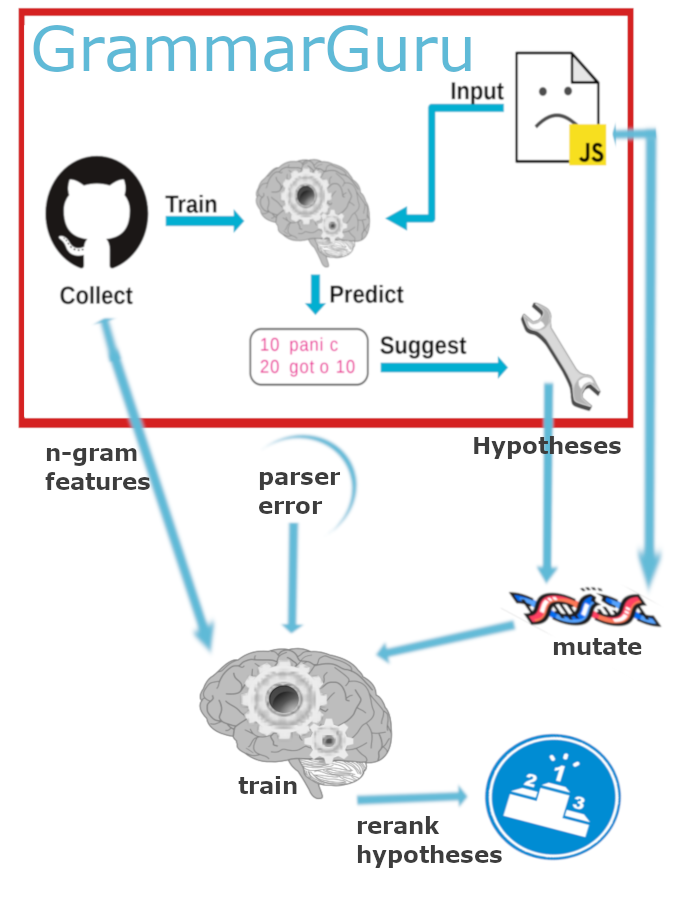
\includegraphics[width=0.8\linewidth]{proj_img}
\end{center}
\section*{Re-ranking}
15 of the most unnatural tokens in the erroneous JS file are fed to our neural network and re-ranked using the ROSE approach. We perform $15 \choose^{2}$ comparisons per file....

%----------------------------------------------------------------------------------------
%	Improving GrammarGuru suggestions
%----------------------------------------------------------------------------------------

\section*{Evaluation}

\section*{References}
\large
$[1]$ \textbf{Santos EA, Campbell JC, Hindle A, Amaral JN. 2017}. Finding and correcting syntax errors using recurrent neural networks. PeerJ Preprints 5:e3123v1 https://doi.org/10.7287/peerj.preprints.3123v1
\\
\\
$[2]$ \textbf{Xingyi Song and Trevor Cohn. 2011}. Regression and ranking based optimisation for sentence level machine translation evaluation. In Proceedings of the Sixth Workshop on Statistical Machine Translation, pages 123–129. Association for Computational Linguistics
\end{multicols}
\end{document}
